\chapter{Prototyp urządzenia}
\label{cha:prototyp}

Głównym zagadnieniem pracy było stworzenie kompletnego urządzenia, które wykryje niebezpieczne zdarzenie i poinformuje o tym zdefiniowanego użytkownika. W niniejszym rozdziale, przeprowadzono testy, mające pomóc stworzyć odpowiednie algorytmy. Opisano również kolejne kroki procesu tworzenia urządzenia, a także rozważono różne podejścia w rozwiązaniu problemów. Omówione zostały również poszczególne fragmenty działającego urządzenia.
%---------------------------------------------------------------------------

Tę część pracy, rozpoczęto od przeprowadzenia podstawowych eksperymentów, mających pokazać, jakich przyspieszeń można spodziewać się w przypadku rzeczywistego zderzenia na rowerze. Testy, rozpoczęo od stworzenia urządzenia, mającgo zbierać surowe dane z akcelerometru. Ze względu na łatwość i szybkość implementacji, wykorzystano platformę Raspberry Pi Zero W, z systemem operacyjnym Raspbian Lite. Korzystając z gotowch bibliotek, napisany został skrypt, który po uruchomieniu tworzył plik tekstowy, do którgo zapisywał surowe dane, pobrane z akcelerometru. Sam akcelerometr, ustawiony był na częstotliwość próbkowania 416Hz i skalę $\pm$8g. 
\newline
Ze względów czysto praktycznych, tj. w celu zabezpieczenia płytek przed uszkodzeniem, wykonany został model 3D prostej obudowy, który został następnie wydrukowany na drukarce 3D. Rysunek \ref{img:test_device_a} przedstawia Raspberry wykonanej na potrzeby projektu obudowie. Zgodnie z rysunkami technicznymi płytki, wykorzystano otwory montażowe. Następnie, stworzono dodatkową warstwę izolacyjną między płytkami, do której przymontowano płytkę z akcelerometrem.(Rysunek \ref{img:test_device_b}) Gotowy układ, zasilany był przy użyciu powerbanku, połączonego przez USB. Obudowa, zamknięta była drukowaną pokrywką. Rozwiązanie przedstawia rysunek \ref{img:test_device_c}.
\newline


\section{Opracowanie algorytmu wykrywania kolizji}
Cały układ, zasilany był przy użyciu zewnętrznej baterii, zamontowanej na siodełku roweru. Ze względu na bezpieczeństwo, testy przeprowadzane były na rowerze bez rowerzysty. Sam układ, zamontowany został na rurze podsiodłowej. Ponieważ jest to prawie centralny punkt roweru, oczekiwano, że przyspieszenia w przypadku silnego wyrzucenia koła w powietrze, będą mniejsze. Eksperyment przeprowadzono przez rozpędzenie roweru do  prędkości około 10$\frac{km}{h}$. Kolejno wykonano:
\begin{itemize}
    \item Zderzenie roweru z drzewem
    \item Upadek na kamieniach
    \item Upadek ze stromego zbocza
\end{itemize}
%TODO: Podmienić zdjęcie urządzenia testowego
\begin{figure}[h]
    \centering
    \begin{subfigure}{3.5cm}
        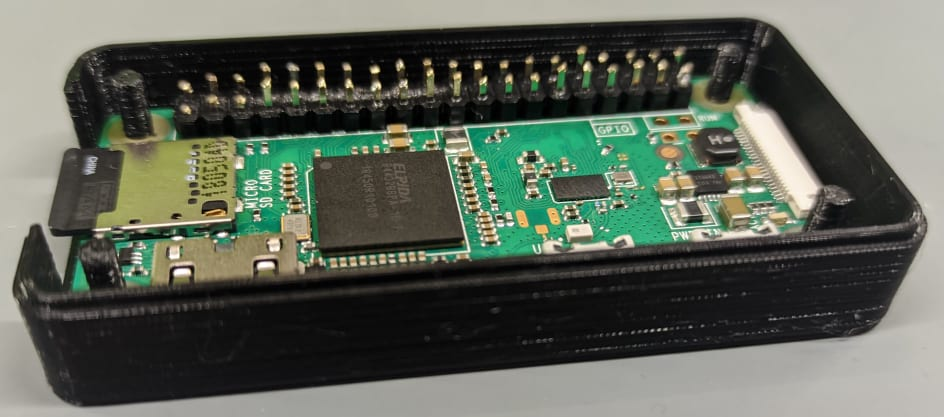
\includegraphics[width=7cm, angle=-90]{Graphics/pi.jpg}
        \caption{Raspberry Pi Zero w drukowanej obudowie}
        \label{img:test_device_a}
    \end{subfigure}
    \begin{subfigure}{3.5cm}
        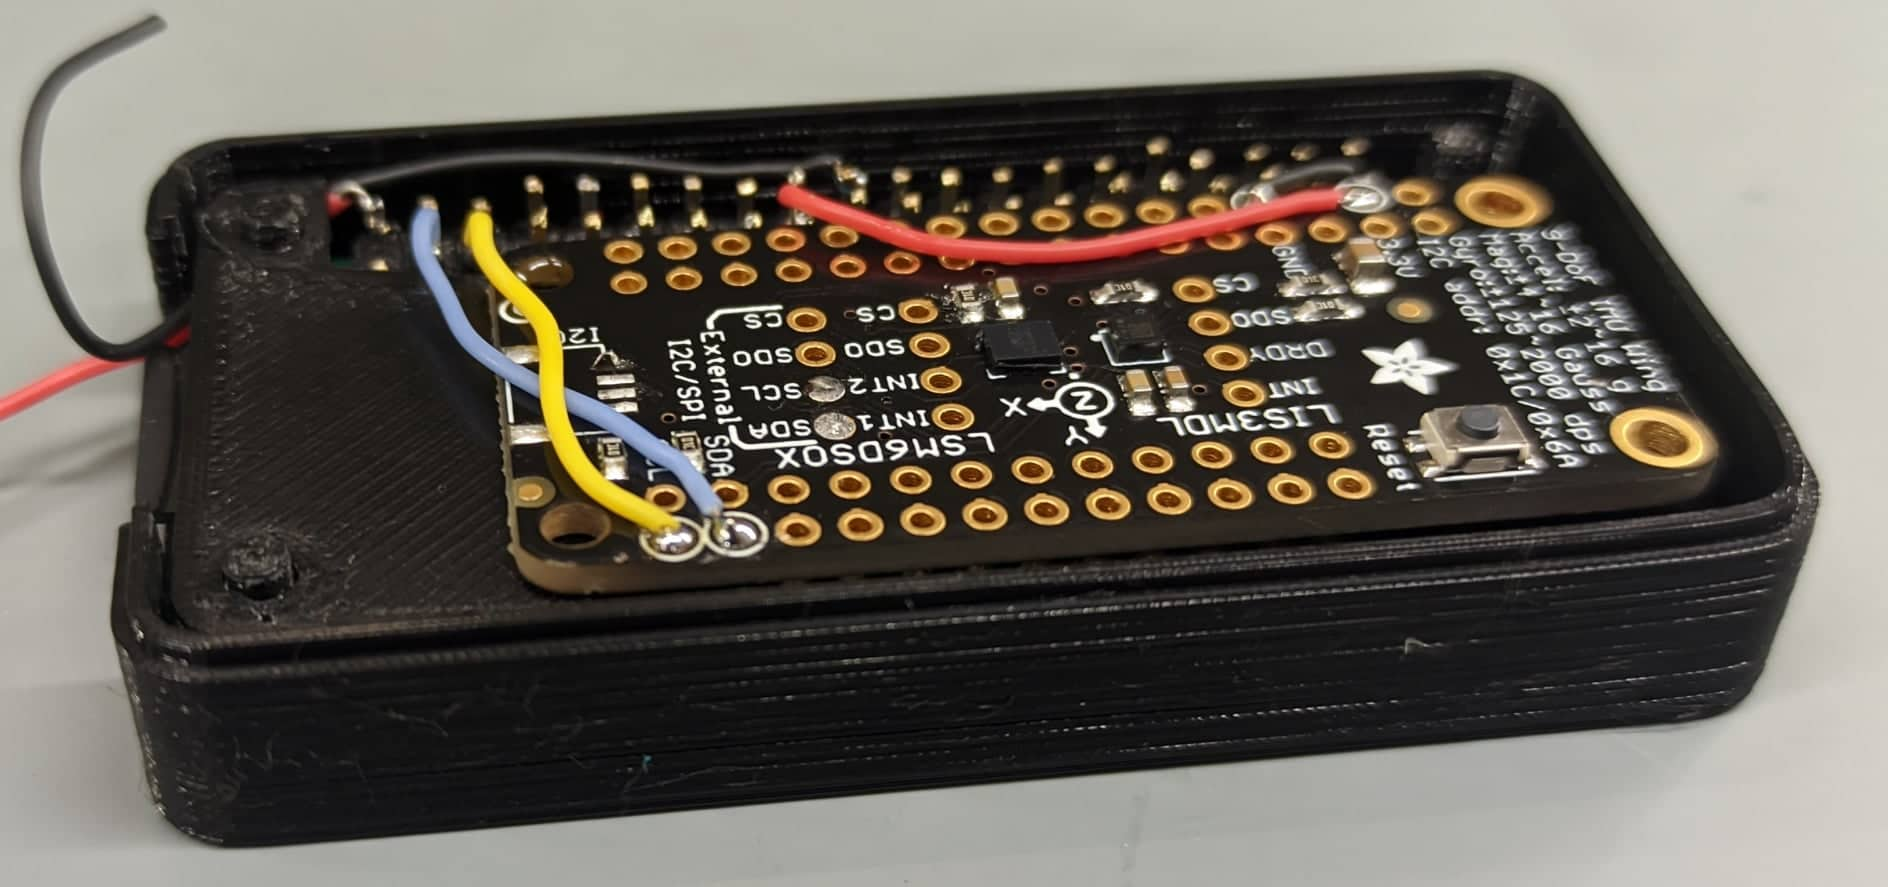
\includegraphics[width=7cm, angle=-90]{Graphics/Pi_acc.jpg}
        \caption{Płytka z akcelerometrem w obudowie}
        \label{img:test_device_b}
    \end{subfigure}
    \begin{subfigure}{3.5cm}
        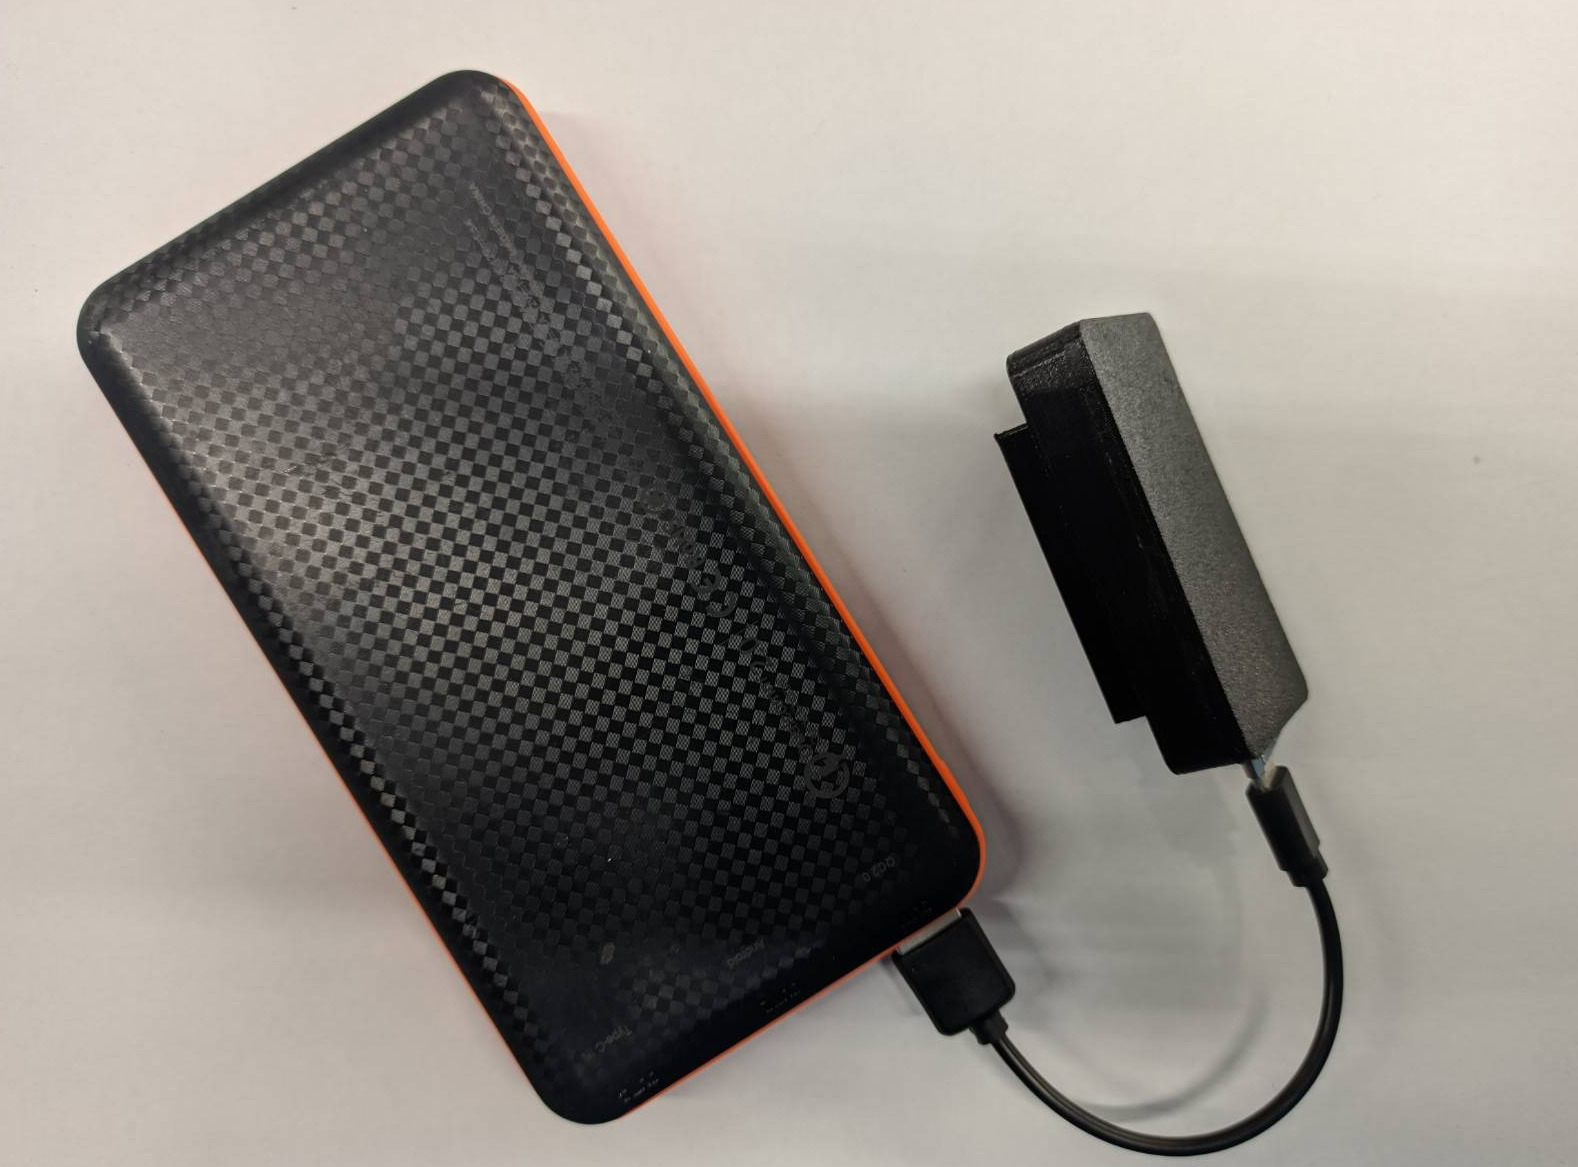
\includegraphics[width=7cm, angle=-90]{Graphics/test_device.jpg}
        \caption{Urządzenie testowe zasilane zewnętrzną baterią}
        \label{img:test_device_c}
    \end{subfigure}
    \caption{Urządzenie testowe do zbierania danych}
\end{figure}

\subsection{Analiza zebranych danych }
\label{sec:data_analysis}
W celu analizy danych, stworzono prosty skrypt w języku Python. Pobierał on surowe dane z pliku, przetwarzał, a następnie rysował zależności czasowe $a(t)$ dla każdej z osi. Ponieważ akcelerometr zwraca liczbę 16-bitową ze znakiem, należało uwzględnić ten fakt w konwersji, ponieważ Python posiada dynamiczne typy danych, co mogło zakłamać wyniki. Zebrane dane, okazały się być znacząco zaszumione. Z tego powodu, przefiltrowane zostały filtrem dolnoprzepustowym. Rysunek \ref{img:bike} przedstawia orientację urządzenia na rowerze. W trakcie analizy danych, przyjęto zaznaczone na nim kierunki osi.
\begin{figure}[hb]
    \centering
    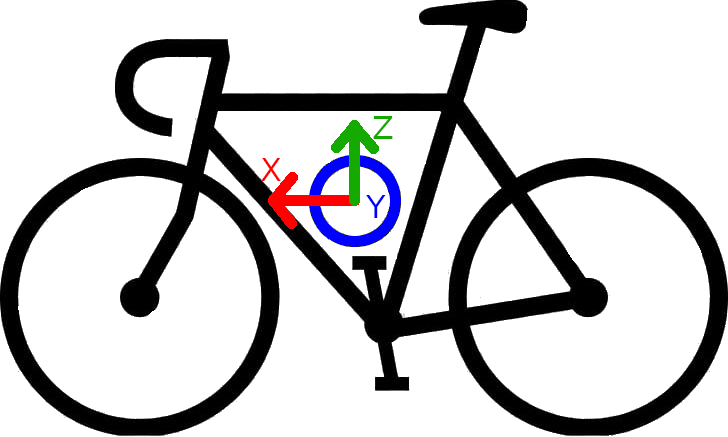
\includegraphics[width=8cm]{Graphics/rowerek.png}
    \caption{Orientacja urządzenia zamontowanego na rowerze}
    \label{img:bike}
\end{figure}
Podczas każdego z testów, rower z przymocowanym urządzeniem, rozpędzono do około 1$\frac{m}{s}$. Zgodnie z przewidywaniami, w większości przypadków, przyspieszenia układu sięgały ok. 1g. Należało również zwrócić uwagę na zwroty przyspieszeń, które zmieniały się po obrocie roweru. Poniżej przedstawiono trzy analizowane przebiegi, na podstawie których utworzone zostały algorytmy. 
\newline
\newline
Rysunek \ref{img:slope} przedstawia zapis upadku ze stromego zbocza. Jest to przypadek gdy rowerzysta górski podczas uskoku, traci kontrolę nad rowerem, lub wypada z trasy. Przez około pół sekundy rower swobodnie spadał, powoli przechylając się w kierunku przedniego koła. Około szóstej sekundy uderzył nim o zbocze, co widać wyraźnie zarówno na osi X, jak i Z. Następnie odbity rower ponownie uderzył w ziemię, tym razem pochylając się po odbiciu na bok. Kolejne uderzenie, było więc uderzeniem bocznym, widocznym jako głęboki dół  na osi Y. Niemal natychmiast, rower obrócił się kołami do góry, co widać na osi Z jako przyspieszenie równe -1g. Po siódmej sekundzie rower zaczął sunąć bokiem wzdłuż zbocza i szybko wyhamowywać. akcelerometr zarejestrował to jako oscylajcje na osi Y pomiędzy 7, a 8 sekundą. Na wykresie, można było również zauważyć, że po zdarzeniu, rower zatrzymał się na jednym z boków, ponieważ oś Y miała stałą wartość bliską 1g.
\newline
\newline
Kolejny z rysunków (\ref{img:stones}), przedstawia sytuację gdy rowerzysta jadąc po kamieniach, uderza tylnym kołem o jeden z nich i traci kontrolę nad rowerem. Sytuacja ta charakterysuje się silnymi oscylacjami osi X i Z, przy względnie stabilnej osi Y. W czwartej sekundzie, rower uderzył tylnym kołem w kamień. Koło zostało wyrzucone do góry, z przyspieszeniem około 1g. Po 500ms rowerzysta rower uderzył z całą energią przednim kołem w ścieżkę, osiągając przyspieszenie prawie 2g. W tej chwili pojazd testowy jeszcze raz odbił się od, a następnie bokiem uderzył w drzewo przy scieżce.
\newline
\newline
Rysunek \ref{img:tree} przedstawia sytuację, gdy rowerzysta tracąc kontrolę nad rowerem, uderza w drzewo. W tym przypadku rower po około 4.5s uderza w drzewo, co odczytane zostało jako wzrost do 0.5g na osi X. Niestety, nie było to uderzenie czyste, ponieważ duża część energii rozłożyła się na odbicie roweru od drzewa. Zapis osi Y pokazuje, że po uderzeniu, rower zaczął obracać się. Ostatecznie jednak, zatrzymał się na jednym z boków.
\newline
\newline
Przeprowadzone testy, pozwoliły na sprawdzenie przeciążeń działających na rower w trakcie wypadku. Pierwszym z nasuwających się wniosków był fakt, że niepotrzebnie ograniczona została częstotliwość próbkowania akcelerometru. W przypadku Raspberry Pi, magistrala I$^{2}$C, pozwala na transmisję 12,5kB/s. Ponieważ jeden zestaw danych zawierał 12 bajtów, częstotliwość próbkowania mogła wynosić aż 1kHz. Tymczasem, ustawiona została częstotliwość 416Hz. Ustawienie to wynikało z obawy, że kod w języku skryptowym nie nadąży za większą częstotliwością. Kolejnym z wniosków, była konieczność stosowania filtrów dolnoprzepustowych. Surowe zapisy z akcelerometru, były silnie zaszumione, na co również wpływ mogła mieć mała częstotliwość próbkowania względem szybkości zmian podczas wypadku. Mimo tego, testy dostarczyły cennych danych na podstawie których stworzono algorytmy, opisane w podrozdziale \ref{sec:state_machines}

%%%%%%%%% Zapisy upadku - wykresy %%%%%%%%%%
\begin{figure}[H]
    \centering
    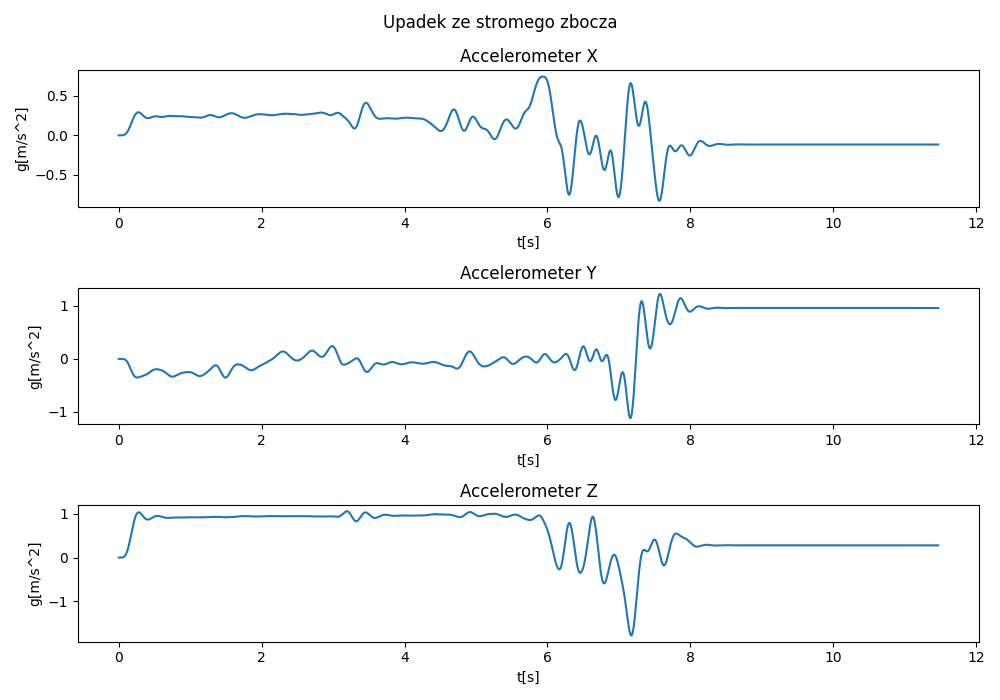
\includegraphics[width=15cm]{Graphics/slope_title.png}
    \caption{Przefiltrowany zapis upadku roweru ze stromego zbocza}
    \label{img:slope}
    \vspace{0.5cm}
    \centering
    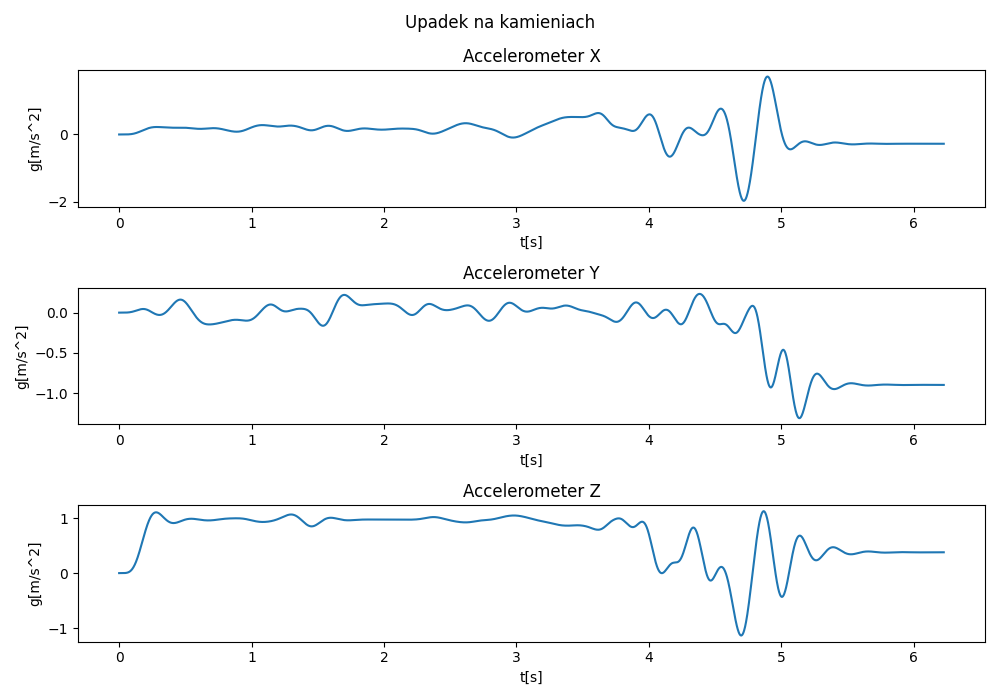
\includegraphics[width=15cm]{Graphics/Stones_title.png}
    \caption{Przefiltrowany zapis upadku roweru na kamieniach}
    \label{img:stones}
\end{figure}
\begin{figure}[h]
    \centering
    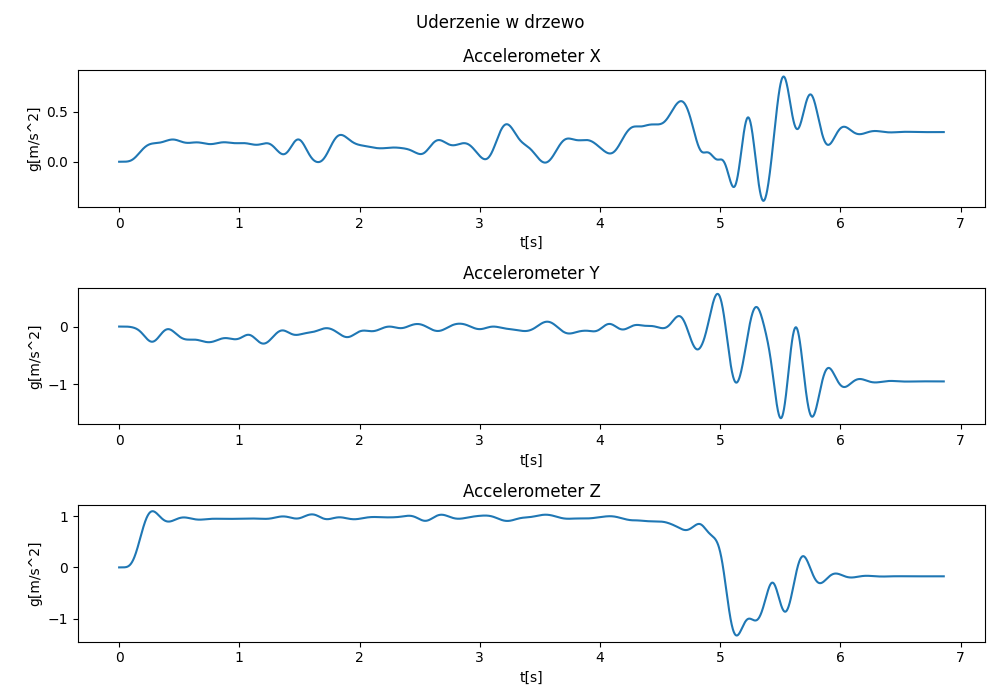
\includegraphics[width=15cm]{Graphics/Tree_title.png}
    \caption{Przefiltrowany zapis uderzenia roweru w drzewo}
    \label{img:tree}
\end{figure}

\subsection{Maszyny stanów wykrywające wypadek}
\label{sec:state_machines}
Na podstawie analizy danych z podrozdziału \ref{sec:data_analysis} zdecydowano się na implementację czterech, niezależnych maszyn stanów. Każda z nich, odpowidać będzie analizowanym przypadkom. Istotnym elementem pracy było możliwie największe uproszczenie maszyn, aby przyspieszyć działanie układu i zminimalizować zużycie energii, bez utraty skuteczności.
\subsubsection{Wykrywanie przeciążenia w dowolnej osi}
Pierwsza z maszyn stanów, służy wykryciu znaczących przeciążeń na dowolnej z osi. Podczas testów zauważono, że podczas każdego z wydarzeń, wysoka wartość przeciążenia odróżnialna była od szumu na podstawie czasu trwania. Określono, że jeśli po około 50ms próbka utrzymuje wysoką wartość, to nastąpiło silne przeciążenie. Ponieważ zdecydowano się skorzystać z wbudowanych w akcelerometr maszyn stanów, można było skorzystać z ich wewnętrznych liczników. Opisywana maszyna stanów, gdy dowolna z osi przekroczy wartość $\pm$6g, ustawia licznik na 50ms. Gdy przez ten czas, nie wystąpi próbka o wartości mniejszej niż 6g, to wyzwolony zostaje alarm. Duża wartość przyspieszenia, pozwoliła uniknąć fałszywych alarmów podczas bezkolizyjnej jazdy. Maszynę przedstawia diagram \ref{img:fsm1}.
\newline
\newline
Dwie kolejne maszyny stanów, przedstawione na diagramie \ref{img:fsm2}, to algorytmy wykrywające przewrócenie roweru. Podczas analizy danych zauważono, że każdy wypadek, kończył się przechyleniem roweru na jeden z boków. Z tego powodu, zaimplementowano licznik, który co 2 sekundy próbkuje wartość na osi Y i sprawdza, czy nie przekracza ona wartości bezwzględnej 0.6g. Jeśli przez dwie minuty, rower nie wróci do pozycji jazdy, wyzwolony zostaje alarm. W praktyce, opisana maszyna musiała zostać zaimplementowana w akcelerometrze jako dwie, niezależne, z uwagi na brak funkcji wartości bezwzględnej w układzie.
\begin{figure}[h]
    \centering
    \begin{subfigure}{4cm}
    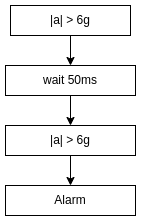
\includegraphics[width=4cm]{Graphics/All_axis_FSM1.png}
    \caption{Wykrycie silnego przeciążenia}
    \label{img:fsm1}
    \end{subfigure}

    \begin{subfigure}{4cm}
    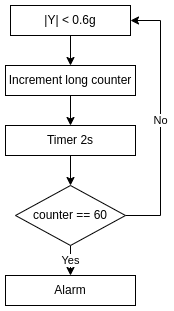
\includegraphics[width=4cm]{Graphics/overturned_FSM2_3.png}
    \caption{Wykrycie przewrócenia roweru}
    \label{img:fsm2}
    \end{subfigure}
    \caption{Maszyny 1-3}
\end{figure}